%%
% Copyright (c) 2017 - 2023, Pascal Wagler;
% Copyright (c) 2014 - 2023, John MacFarlane
%
% All rights reserved.
%
% Redistribution and use in source and binary forms, with or without
% modification, are permitted provided that the following conditions
% are met:
%
% - Redistributions of source code must retain the above copyright
% notice, this list of conditions and the following disclaimer.
%
% - Redistributions in binary form must reproduce the above copyright
% notice, this list of conditions and the following disclaimer in the
% documentation and/or other materials provided with the distribution.
%
% - Neither the name of John MacFarlane nor the names of other
% contributors may be used to endorse or promote products derived
% from this software without specific prior written permission.
%
% THIS SOFTWARE IS PROVIDED BY THE COPYRIGHT HOLDERS AND CONTRIBUTORS
% "AS IS" AND ANY EXPRESS OR IMPLIED WARRANTIES, INCLUDING, BUT NOT
% LIMITED TO, THE IMPLIED WARRANTIES OF MERCHANTABILITY AND FITNESS
% FOR A PARTICULAR PURPOSE ARE DISCLAIMED. IN NO EVENT SHALL THE
% COPYRIGHT OWNER OR CONTRIBUTORS BE LIABLE FOR ANY DIRECT, INDIRECT,
% INCIDENTAL, SPECIAL, EXEMPLARY, OR CONSEQUENTIAL DAMAGES (INCLUDING,
% BUT NOT LIMITED TO, PROCUREMENT OF SUBSTITUTE GOODS OR SERVICES;
% LOSS OF USE, DATA, OR PROFITS; OR BUSINESS INTERRUPTION) HOWEVER
% CAUSED AND ON ANY THEORY OF LIABILITY, WHETHER IN CONTRACT, STRICT
% LIABILITY, OR TORT (INCLUDING NEGLIGENCE OR OTHERWISE) ARISING IN
% ANY WAY OUT OF THE USE OF THIS SOFTWARE, EVEN IF ADVISED OF THE
% POSSIBILITY OF SUCH DAMAGE.
%%

%%
% This is the Eisvogel pandoc LaTeX template.
%
% For usage information and examples visit the official GitHub page:
% https://github.com/Wandmalfarbe/pandoc-latex-template
%%

% Options for packages loaded elsewhere
\PassOptionsToPackage{unicode}{hyperref}
\PassOptionsToPackage{hyphens}{url}
\PassOptionsToPackage{dvipsnames,svgnames,x11names,table}{xcolor}
%
\documentclass[
  paper=a4,
  ,captions=tableheading
]{scrartcl}
\usepackage{amsmath,amssymb}
% Use setspace anyway because we change the default line spacing.
% The spacing is changed early to affect the titlepage and the TOC.
\usepackage{setspace}
%\setstretch{1.2}
\setstretch{1.0}
\usepackage{iftex}
\ifPDFTeX
  \usepackage[T1]{fontenc}
  \usepackage[utf8]{inputenc}
  \usepackage{textcomp} % provide euro and other symbols
\else % if luatex or xetex
  \usepackage{unicode-math} % this also loads fontspec
  \defaultfontfeatures{Scale=MatchLowercase}
  \defaultfontfeatures[\rmfamily]{Ligatures=TeX,Scale=1}
\fi
\usepackage{lmodern}
\ifPDFTeX\else
  % xetex/luatex font selection
\fi
% Use upquote if available, for straight quotes in verbatim environments
\IfFileExists{upquote.sty}{\usepackage{upquote}}{}
\IfFileExists{microtype.sty}{% use microtype if available
  \usepackage[]{microtype}
  \UseMicrotypeSet[protrusion]{basicmath} % disable protrusion for tt fonts
}{}
\makeatletter
\@ifundefined{KOMAClassName}{% if non-KOMA class
  \IfFileExists{parskip.sty}{%
    \usepackage{parskip}
  }{% else
    \setlength{\parindent}{0pt}
    \setlength{\parskip}{6pt plus 2pt minus 1pt}}
}{% if KOMA class
  \KOMAoptions{parskip=half}}
\makeatother
\usepackage{xcolor}
\definecolor{default-linkcolor}{HTML}{A50000}
\definecolor{default-filecolor}{HTML}{A50000}
\definecolor{default-citecolor}{HTML}{4077C0}
\definecolor{default-urlcolor}{HTML}{4077C0}
\usepackage[margin=2.5cm,includehead=true,includefoot=true,centering,]{geometry}
\usepackage{listings}
\newcommand{\passthrough}[1]{#1}
\lstset{defaultdialect=[5.3]Lua}
\lstset{defaultdialect=[x86masm]Assembler}
\usepackage{etoolbox}
\BeforeBeginEnvironment{lstlisting}{\par\noindent\begin{minipage}{\linewidth}}
\AfterEndEnvironment{lstlisting}{\end{minipage}\par\addvspace{\topskip}}
\usepackage{longtable,booktabs,array}
\usepackage{calc} % for calculating minipage widths
% Correct order of tables after \paragraph or \subparagraph
\usepackage{etoolbox}
\makeatletter
\patchcmd\longtable{\par}{\if@noskipsec\mbox{}\fi\par}{}{}
\makeatother
% Allow footnotes in longtable head/foot
\IfFileExists{footnotehyper.sty}{\usepackage{footnotehyper}}{\usepackage{footnote}}
\makesavenoteenv{longtable}
% add backlinks to footnote references, cf. https://tex.stackexchange.com/questions/302266/make-footnote-clickable-both-ways
\usepackage{footnotebackref}
\usepackage{graphicx}
\makeatletter
\def\maxwidth{\ifdim\Gin@nat@width>\linewidth\linewidth\else\Gin@nat@width\fi}
\def\maxheight{\ifdim\Gin@nat@height>\textheight\textheight\else\Gin@nat@height\fi}
\makeatother
% Scale images if necessary, so that they will not overflow the page
% margins by default, and it is still possible to overwrite the defaults
% using explicit options in \includegraphics[width, height, ...]{}
\setkeys{Gin}{width=\maxwidth,height=\maxheight,keepaspectratio}
% Set default figure placement to htbp
\makeatletter
% Make use of float-package and set default placement for figures to H.
% The option H means 'PUT IT HERE' (as  opposed to the standard h option which means 'You may put it here if you like').
\usepackage{float}
\floatplacement{figure}{H}
\makeatother
\setlength{\emergencystretch}{3em} % prevent overfull lines
\providecommand{\tightlist}{%
  \setlength{\itemsep}{0pt}\setlength{\parskip}{0pt}}
\setcounter{secnumdepth}{5}
\ifLuaTeX
  \usepackage{selnolig}  % disable illegal ligatures
\fi
\IfFileExists{bookmark.sty}{\usepackage{bookmark}}{\usepackage{hyperref}}
\IfFileExists{xurl.sty}{\usepackage{xurl}}{} % add URL line breaks if available
\urlstyle{same}
\hypersetup{
  pdftitle={Putting Fortran's object-related features to practical use},
  pdfauthor={Reinhold Bader (1966 - 2024)},
  % hidelinks,
  breaklinks=true,
  pdfcreator={LaTeX via pandoc with an edited Eisvogel template}}
\title{Putting Fortran's object-related features to practical use}
\author{Reinhold Bader (1966 - 2024)}
\date{2024}



%%
%% added
%%


%
% for the background color of the title page
%

%
% break urls
%
\PassOptionsToPackage{hyphens}{url}

%
% When using babel or polyglossia with biblatex, loading csquotes is recommended
% to ensure that quoted texts are typeset according to the rules of your main language.
%
\usepackage{csquotes}

%
% captions
%
\definecolor{caption-color}{HTML}{777777}
\usepackage[font={stretch=1.2}, textfont={color=caption-color}, position=top, skip=4mm, labelfont=bf, singlelinecheck=false, justification=raggedright]{caption}
\setcapindent{0em}

%
% blockquote
%
\definecolor{blockquote-border}{RGB}{221,221,221}
\definecolor{blockquote-text}{RGB}{119,119,119}
\usepackage{mdframed}
\newmdenv[rightline=false,bottomline=false,topline=false,linewidth=3pt,linecolor=blockquote-border,skipabove=\parskip]{customblockquote}
\renewenvironment{quote}{\begin{customblockquote}\list{}{\rightmargin=0em\leftmargin=0em}%
\item\relax\color{blockquote-text}\ignorespaces}{\unskip\unskip\endlist\end{customblockquote}}

%
% Source Sans Pro as the default font family
% Source Code Pro for monospace text
%
% 'default' option sets the default
% font family to Source Sans Pro, not \sfdefault.
%
\ifnum 0\ifxetex 1\fi\ifluatex 1\fi=0 % if pdftex
    % \usepackage[default]{sourcesanspro}
  % \usepackage{sourcecodepro}
  \usepackage{libertine}
  \usepackage{libertinust1math}
  \usepackage[scaled=0.84]{beramono}
  \renewcommand*{\figureformat}{}
  \else % if not pdftex
    \usepackage[default]{sourcesanspro}
  \usepackage{sourcecodepro}

  % XeLaTeX specific adjustments for straight quotes: https://tex.stackexchange.com/a/354887
  % This issue is already fixed (see https://github.com/silkeh/latex-sourcecodepro/pull/5) but the
  % fix is still unreleased.
  % TODO: Remove this workaround when the new version of sourcecodepro is released on CTAN.
  \ifxetex
    \makeatletter
    \defaultfontfeatures[\ttfamily]
      { Numbers   = \sourcecodepro@figurestyle,
        Scale     = \SourceCodePro@scale,
        Extension = .otf }
    \setmonofont
      [ UprightFont    = *-\sourcecodepro@regstyle,
        ItalicFont     = *-\sourcecodepro@regstyle It,
        BoldFont       = *-\sourcecodepro@boldstyle,
        BoldItalicFont = *-\sourcecodepro@boldstyle It ]
      {SourceCodePro}
    \makeatother
  \fi
  \fi

%
% heading color
%
\definecolor{heading-color}{RGB}{40,40,40}
\addtokomafont{section}{\color{heading-color}}
% When using the classes report, scrreprt, book,
% scrbook or memoir, uncomment the following line.
%\addtokomafont{chapter}{\color{heading-color}}

%
% variables for title, author and date
%
\usepackage{titling}
\title{Putting Fortran's object-related features to practical use}
\author{Reinhold Bader (1966 - 2024)}
\date{2024}

%
% tables
%

\definecolor{table-row-color}{HTML}{F5F5F5}
\definecolor{table-rule-color}{HTML}{999999}

%\arrayrulecolor{black!40}
\arrayrulecolor{table-rule-color}     % color of \toprule, \midrule, \bottomrule
\setlength\heavyrulewidth{0.3ex}      % thickness of \toprule, \bottomrule
\renewcommand{\arraystretch}{1.3}     % spacing (padding)


%
% remove paragraph indentation
%
\setlength{\parindent}{0pt}
\setlength{\parskip}{6pt plus 2pt minus 1pt}
\setlength{\emergencystretch}{3em}  % prevent overfull lines

%
%
% Listings
%
%


%
% general listing colors
%
\definecolor{listing-background}{HTML}{F7F7F7}
\definecolor{listing-rule}{HTML}{B3B2B3}
\definecolor{listing-numbers}{HTML}{B3B2B3}
\definecolor{listing-text-color}{HTML}{000000}
\definecolor{listing-keyword}{HTML}{435489}
\definecolor{listing-keyword-2}{HTML}{1284CA} % additional keywords
\definecolor{listing-keyword-3}{HTML}{9137CB} % additional keywords
\definecolor{listing-identifier}{HTML}{435489}
\definecolor{listing-string}{HTML}{00999A}
\definecolor{listing-comment}{HTML}{8E8E8E}

\lstdefinestyle{eisvogel_listing_style}{
  language         = java,
  xleftmargin      = 0.6em,
  framexleftmargin = 0.4em,
  backgroundcolor  = \color{listing-background},
  basicstyle       = \color{listing-text-color}\linespread{1.0}%
                      \lst@ifdisplaystyle%
                      \small%
                      \fi\ttfamily{},
  breaklines       = true,
  frame            = single,
  framesep         = 0.19em,
  rulecolor        = \color{listing-rule},
  frameround       = ffff,
  tabsize          = 4,
  numberstyle      = \color{listing-numbers},
  aboveskip        = 1.0em,
  belowskip        = 0.1em,
  abovecaptionskip = 0em,
  belowcaptionskip = 1.0em,
  keywordstyle     = {\color{listing-keyword}\bfseries},
  keywordstyle     = {[2]\color{listing-keyword-2}\bfseries},
  keywordstyle     = {[3]\color{listing-keyword-3}\bfseries\itshape},
  sensitive        = true,
  identifierstyle  = \color{listing-identifier},
  commentstyle     = \color{listing-comment},
  stringstyle      = \color{listing-string},
  showstringspaces = false,
  escapeinside     = {/*@}{@*/}, % Allow LaTeX inside these special comments
  literate         =
  {á}{{\'a}}1 {é}{{\'e}}1 {í}{{\'i}}1 {ó}{{\'o}}1 {ú}{{\'u}}1
  {Á}{{\'A}}1 {É}{{\'E}}1 {Í}{{\'I}}1 {Ó}{{\'O}}1 {Ú}{{\'U}}1
  {à}{{\`a}}1 {è}{{\`e}}1 {ì}{{\`i}}1 {ò}{{\`o}}1 {ù}{{\`u}}1
  {À}{{\`A}}1 {È}{{\`E}}1 {Ì}{{\`I}}1 {Ò}{{\`O}}1 {Ù}{{\`U}}1
  {ä}{{\"a}}1 {ë}{{\"e}}1 {ï}{{\"i}}1 {ö}{{\"o}}1 {ü}{{\"u}}1
  {Ä}{{\"A}}1 {Ë}{{\"E}}1 {Ï}{{\"I}}1 {Ö}{{\"O}}1 {Ü}{{\"U}}1
  {â}{{\^a}}1 {ê}{{\^e}}1 {î}{{\^i}}1 {ô}{{\^o}}1 {û}{{\^u}}1
  {Â}{{\^A}}1 {Ê}{{\^E}}1 {Î}{{\^I}}1 {Ô}{{\^O}}1 {Û}{{\^U}}1
  {œ}{{\oe}}1 {Œ}{{\OE}}1 {æ}{{\ae}}1 {Æ}{{\AE}}1 {ß}{{\ss}}1
  {ç}{{\c c}}1 {Ç}{{\c C}}1 {ø}{{\o}}1 {å}{{\r a}}1 {Å}{{\r A}}1
  {€}{{\EUR}}1 {£}{{\pounds}}1 {«}{{\guillemotleft}}1
  {»}{{\guillemotright}}1 {ñ}{{\~n}}1 {Ñ}{{\~N}}1 {¿}{{?`}}1
  {…}{{\ldots}}1 {≥}{{>=}}1 {≤}{{<=}}1 {„}{{\glqq}}1 {“}{{\grqq}}1
  {”}{{''}}1
}
\lstset{style=eisvogel_listing_style}

%
% Java (Java SE 12, 2019-06-22)
%
\lstdefinelanguage{Java}{
  morekeywords={
    % normal keywords (without data types)
    abstract,assert,break,case,catch,class,continue,default,
    do,else,enum,exports,extends,final,finally,for,if,implements,
    import,instanceof,interface,module,native,new,package,private,
    protected,public,requires,return,static,strictfp,super,switch,
    synchronized,this,throw,throws,transient,try,volatile,while,
    % var is an identifier
    var
  },
  morekeywords={[2] % data types
    % primitive data types
    boolean,byte,char,double,float,int,long,short,
    % String
    String,
    % primitive wrapper types
    Boolean,Byte,Character,Double,Float,Integer,Long,Short
    % number types
    Number,AtomicInteger,AtomicLong,BigDecimal,BigInteger,DoubleAccumulator,DoubleAdder,LongAccumulator,LongAdder,Short,
    % other
    Object,Void,void
  },
  morekeywords={[3] % literals
    % reserved words for literal values
    null,true,false,
  },
  sensitive,
  morecomment  = [l]//,
  morecomment  = [s]{/*}{*/},
  morecomment  = [s]{/**}{*/},
  morestring   = [b]",
  morestring   = [b]',
}

\lstdefinelanguage{XML}{
  morestring      = [b]",
  moredelim       = [s][\bfseries\color{listing-keyword}]{<}{\ },
  moredelim       = [s][\bfseries\color{listing-keyword}]{</}{>},
  moredelim       = [l][\bfseries\color{listing-keyword}]{/>},
  moredelim       = [l][\bfseries\color{listing-keyword}]{>},
  morecomment     = [s]{<?}{?>},
  morecomment     = [s]{<!--}{-->},
  commentstyle    = \color{listing-comment},
  stringstyle     = \color{listing-string},
  identifierstyle = \color{listing-identifier}
}

%
% header and footer
%
\usepackage[headsepline,footsepline]{scrlayer-scrpage}

\newpairofpagestyles{eisvogel-header-footer}{
  \clearpairofpagestyles
  \ihead*{Putting Fortran's object-related features to practical use}
  \chead*{}
  \ohead*{2024}
  \ifoot*{Reinhold Bader (1966 - 2024)}
  \cfoot*{}
  \ofoot*{\thepage}
  \addtokomafont{pageheadfoot}{\upshape}
}
\pagestyle{eisvogel-header-footer}



%%
%% end added
%%

\begin{document}

%%
%% begin titlepage
%%

%%
%% end titlepage
%%

% \maketitle


{
\setcounter{tocdepth}{3}
\tableofcontents
}
This article describes how advanced Fortran language features can be
applied toward object-based and object-oriented programming techniques.
These are, of course, to a significant extent a matter of taste,
personal style and possibly overarching program design considerations,
so should be taken with a pinch of salt.

Language features from Fortran 95 and later will be used; those from
Fortran 2003 and later will also be shortly described. They are
explained in more detail in e.g., Metcalf, Reid, Cohen and
Bader.\footnote{Metcalf, Michael; Reid, John; Cohen, Malcolm; Bader,
  Reinhold (2023). \emph{Modern Fortran Explained.} Numerical
  Mathematics and Scientific Computation. Oxford University Press.
  \href{https://en.wikipedia.org/wiki/Special:BookSources/978-0-19-887657-1}{ISBN
  978-0-19-887657-1}.} See also
\href{https://en.wikipedia.org/wiki/Fortran_95_language_features}{Fortran
95 language features} for the language's fundamentals; the prerequisite
for understanding this article is that features explained there are well
understood.

Boldface will be used where term definitions are introduced. They are
additionally annotated by ``(not a Fortran term)'' or similar if the
term is not used in the Fortran standard itself, but is in general use
in the technical literature.

Compilable and runnable example code is available from an external
\href{https://github.com/reinh-bader/object_fortran}{Github repository}.

\section{Object-based programming techniques}\label{sec:oop_techniques}

\section{Introduction: Container-like
types}\label{introduction-container-like-types}

The word ``Container-like'' is not a Fortran term, but used in the
context of this article to designate types with components whose size
(or type, to be discussed later) is not known when the type is declared.
For deferred sizing of array objects, this can be achieved by using
either the \passthrough{\lstinline!POINTER!} or the
\passthrough{\lstinline!ALLOCATABLE!} attribute for the component's
specification.

The language features and programming techniques will be shown using two
examples introduced in the following section. The demonstration codes
for this chapter can be found in the
\passthrough{\lstinline!object\_based!} folder of the
\href{https://github.com/reinh-bader/object_fortran}{Github repository}.

\section{Examples for definitions of container-like
types}\label{examples-for-definitions-of-container-like-types}

\subsection{Allocatable components}\label{allocatable-components}

As an example for the type definition of a \textbf{value container} (not
a Fortran term) with an \passthrough{\lstinline!ALLOCATABLE!} component
consider

\begin{lstlisting}
TYPE :: polynomial
   PRIVATE
   REAL, ALLOCATABLE :: a(:)
END TYPE
\end{lstlisting}

An object declared to be of this type

\begin{lstlisting}
TYPE(polynomial) :: p
\end{lstlisting}

is suitable for characterization of a polynomial

\(p(x) = \sum_{k=0}^{\text{degree}} a_{k} \cdot x^k \quad (x \in \Re)\)

once it has been created and subsequently supplied with values of the
coefficients:

\begin{lstlisting}
degree = ... ! integer value known at run time only
ALLOCATE( p%a(0:degree) )
p%a(0:) = ...
\end{lstlisting}

\subsection{Pointer components}\label{pointer-components}

As an example for the type definition of a \textbf{reference container}
(not a Fortran term) with a \passthrough{\lstinline!POINTER!} component
consider

\begin{lstlisting}
TYPE :: sorted_list
   PRIVATE
   TYPE(sortable) :: data
   TYPE(sorted_list), POINTER :: next => null()
END TYPE
\end{lstlisting}

Note that referencing the type itself when declaring a component is
permitted if that component has the \passthrough{\lstinline!POINTER!} or
\passthrough{\lstinline!ALLOCATABLE!} attribute; such types are
generally known as \textbf{recursive}. They are used to represent
information structures (lists, trees, \ldots), often with specific
relationships between the individual data entries stored in each node.
In this example, the assumption is that entries of type
\passthrough{\lstinline!data!} in subsequent list items fulfill an
ordering condition, based on the functionality supplied with that type:

\begin{lstlisting}
TYPE, PUBLIC :: sortable
   CHARACTER(len=:), ALLOCATABLE :: string
END TYPE

INTERFACE OPERATOR(<)          ! compare two objects of type sortable
   MODULE PROCEDURE less_than  ! implementation not shown here
END INTERFACE
\end{lstlisting}

Given that Fortran supports arrays, use of simple linked lists is in
most cases inappropriate. The example is presented here as being the
simplest that permits illustrating the language features of interest.

An object declared to be

\begin{lstlisting}
TYPE(sorted_list) :: my_list
\end{lstlisting}

is suitable as starting point for building a linked list with node
entries of type \passthrough{\lstinline!data!}. In the simplest case,
inserting a data item into the object is done by executing the following
statements:

\begin{lstlisting}
TYPE(sortable) :: my_data
:
my_data = ...
my_list%data = my_data  ! only compiles if type definition is accessible in host
\end{lstlisting}

However, as we shall see below, setting up a complete and valid
\passthrough{\lstinline!sorted\_list!} object in a reliable manner needs
additional work.

\section{Constructing objects of container-like
type}\label{constructing-objects-of-container-like-type}

The semantics of the default structure constructor for container-like
objects needs to account for any additional
\passthrough{\lstinline!POINTER!} or
\passthrough{\lstinline!ALLOCATABLE!} attribute specified for type
components.

For the first example type from the last section, the executable
statements in

\begin{lstlisting}
TYPE(polynomial) :: q, r
:
q = polynomial( [2., 3., 1.] )
r = polynomial( null() )
\end{lstlisting}

result in an object \passthrough{\lstinline!q!} auto-allocated to the
value \passthrough{\lstinline!q\%a(1:3) == [2., 3., 1.]!}, and an object
\passthrough{\lstinline!r!} with \passthrough{\lstinline!r\%a!}
unallocated.

For the second example type from the last section, the executable
statements in

\begin{lstlisting}
TYPE(sorted_list) :: sl1
TYPE(sorted_list), target :: sl2
TYPE(sortable) :: d1, d2
:
sl1 = sorted_list( data=d1, next=sl2 )  ! use keyword notation
sl2 = sorted_list( d2, null() )
\end{lstlisting}

result in an object \passthrough{\lstinline!sl1!} with
\passthrough{\lstinline!sl1\%next!} pointer associated with
\passthrough{\lstinline!sl2!}, and an object
\passthrough{\lstinline!sl2!} with \passthrough{\lstinline!sl2\%next!}
disassociated; the \passthrough{\lstinline!data!} components of both
objects have values, \passthrough{\lstinline!d1!} and
\passthrough{\lstinline!d2!}, respectively. Note that an argument that
matches with a \passthrough{\lstinline!POINTER!} component must have
either the \passthrough{\lstinline!POINTER!} or the
\passthrough{\lstinline!TARGET!} attribute. Also, \textbf{keyword
notation} can be used in structure constructors in the same manner as
for procedure arguments.

The default constructor's behaviour has some properties that one needs
to be aware of:

\begin{enumerate}
\def\labelenumi{\arabic{enumi}.}
\tightlist
\item
  If all type components have the \passthrough{\lstinline!PRIVATE!}
  attribute i.e., the type is \textbf{opaque} (not a Fortran term), it
  can only be used if the type declaration is accessed by host
  association (this is the same as for nonallocatable/nonpointer
  components);
\item
  especially for container-like types, its semantics may be incompatible
  with the programmers intentions for how the objects should be used.
\end{enumerate}

Item 2 is illustrated by the above object setups, specifically:

\begin{itemize}
\tightlist
\item
  In the \passthrough{\lstinline!polynomial!} example given above, the
  lower bound of \passthrough{\lstinline!q\%a!} is set to 1, contrary to
  the expectation that it should be 0. One could account for this by
  calculating index offsets in any module procedures that process
  \passthrough{\lstinline!polynomial!} objects, but this makes the code
  harder to understand and maintain. Also, the degree of the polynomial
  should be determined by the last nonzero entry of the coefficient
  array, but the language can of course not be aware of this.
\item
  In the \passthrough{\lstinline!sorted\_list!} example given above, the
  ordering requirement for entries in subsequent nodes is not checked,
  so will usually be not fulfilled. Also, if
  \passthrough{\lstinline!sl2!} goes out of scope before
  \passthrough{\lstinline!sl1!} does, the list structure is torn to
  bits.
\end{itemize}

The programmer can enforce appropriate semantics by overloading the
structure constructor. In this case, it is usually a good idea to
declare the types as being opaque.

Overloading the structure constructor is done by

\begin{itemize}
\tightlist
\item
  creating a named interface (i.e., a generic function) with the same
  name as the type of interest;
\item
  creating at least one specific function (a subroutine is not
  permitted), usually returning a scalar result of the type of interest.
\end{itemize}

For the \passthrough{\lstinline!polynomial!} type the interface block
(placed in the specification section of the module containing the type
definition) might read

\begin{lstlisting}
INTERFACE polynomial
! overload to assure correct lower bound when creating a polynomial object
   MODULE PROCEDURE :: create_polynomial
   ... ! further specifics as needed
END INTERFACE
\end{lstlisting}

and the implementation of \passthrough{\lstinline!create\_polynomial!}
(in the \passthrough{\lstinline!CONTAINS!} part of the module) might
read

\begin{lstlisting}
PURE TYPE(polynomial) FUNCTION create_polynomial(a)
   REAL, INTENT(in) :: a(0:)
   INTEGER :: degree(1)

   degree = findloc( a /= 0.0, value=.true., back=.true. ) - 1
   ALLOCATE( create_polynomial%a(0:degree(1)) )
   create_polynomial%a(0:) = a(0:degree(1))
END FUNCTION
\end{lstlisting}

Because its signature matches the default structure constructor's, the
function actually overrides the default constructor, making it generally
unavailable.

For the \passthrough{\lstinline!sorted\_list!} type the interface block
might read

\begin{lstlisting}
INTERFACE sorted_list
! the default constructor is unavailable because the type is opaque
! the specific has a different signature than the structure constructor
   MODULE PROCEDURE :: create_sorted_list
   ... ! further specifics as needed
END INTERFACE
\end{lstlisting}

with the implementation of
\passthrough{\lstinline!create\_sorted\_list!} as follows:

\begin{lstlisting}
PURE FUNCTION create_sorted_list(item_array) RESULT(head)
   TYPE(sortable), INTENT(in) :: item_array(:)
   TYPE(sorted_list) :: head
   INTEGER :: i

   DO i = 1, size(item_array)
      CALL add_to_sorted_list(head, item_array(i))
      ! handles tedious details of pointer fiddling
   END DO
END FUNCTION
\end{lstlisting}

The constructor has a signature that differs from that of the default
one, but the latter is unavailable outside the host scope of the type
definition anyway, due to the opacity of
\passthrough{\lstinline!sorted\_list!}.

\section{Copying objects of container-like
type}\label{copying-objects-of-container-like-type}

Default assignment extends to container-like objects. For objects
declared as

\begin{lstlisting}
TYPE(polynomial) :: p, q
TYPE(sorted_list) :: slp, slq

... ! code that defines p, slp
\end{lstlisting}

and after defining values for prospective right-hand sides, execution of
the statement

\begin{lstlisting}
q = p
\end{lstlisting}

produces the same result as

\begin{lstlisting}
IF ( allocated(q%a) ) DEALLOCATE( q%a )
q%a = p%a  ! performs auto-allocation using the RHS's bounds, then copies the value
\end{lstlisting}

and execution of the statement

\begin{lstlisting}
slq = slp
\end{lstlisting}

produces the same result as

\begin{lstlisting}
slq%data = slp%data
slq%next => slp%next  ! creates a reference between list objects without copying any value
\end{lstlisting}

The terms \textbf{deep copy} and \textbf{shallow copy} (neither are
Fortran terms) are sometimes used to describe the above behaviour for
\passthrough{\lstinline!ALLOCATABLE!} and
\passthrough{\lstinline!POINTER!} components, respectively. Note that -
different from the default structure constructor - having
\passthrough{\lstinline!PRIVATE!} components does not affect the use of
default assigment. However, the semantics of default assignment might
not be what is needed from the programmer's point of view.

Specifically, consider the case where the object
\passthrough{\lstinline!slq!} above has previously been set up by
invoking the overloaded constructor. The assignment above would then
have the following effects:

\begin{enumerate}
\def\labelenumi{\arabic{enumi}.}
\tightlist
\item
  The list elements of the original \passthrough{\lstinline!slq!},
  beginning with \passthrough{\lstinline!slq\%next!}, would become
  inaccessible (``orphaned''), effectively causing a memory leak;
\item
  after the assignment statement, \passthrough{\lstinline!slq\%next!}
  references into \passthrough{\lstinline!slp\%next!}, resulting in
  aliasing.
\end{enumerate}

To avoid 2., it is possible to
\href{https://en.wikipedia.org/wiki/Fortran_95_language_features\#Derived-data_types}{\textbf{overload}
the assignment operator} for reference containers to create a deep copy.
Note that in the case where defined unary or binary operations are
introduced, the functions that define these need to create deep copies
to create the result variable anyway, otherwise things simply don't
work. The downside of this is that in code like

\begin{lstlisting}
slq = slp // slq
\end{lstlisting}

~- with the overloaded concatenation operator meaning that the argument
lists are joined - multiple deep copies need to be done (the
implementation of the module procedure
\passthrough{\lstinline!join\_lists!} that supplies the necessary
specific for \passthrough{\lstinline!//!} is not shown here; see the
source \passthrough{\lstinline!code sorted\_list.f90!} for details). It
turns out that some of these exist only intermediately.

Here an implementation of the specific procedure for the overloaded
assignment of \passthrough{\lstinline!sorted\_list!} objects:

\begin{lstlisting}
SUBROUTINE assign_sorted_list(to, from)
   TYPE(sorted_list), INTENT(in), TARGET :: from
   TYPE(sorted_list), INTENT(out), TARGET :: to  ! finalizer is executed on entry,
                                                 ! see below for discussion of this.
   TYPE(sorted_list), POINTER :: p, q

   p => from; q => to

   deep_copy : DO
      IF ( associated(p) ) THEN
         q%data = p%data
      ELSE
         EXIT deep_copy
      END IF
      p => p%next
      IF ( associated(p) ) ALLOCATE( q%next )
      q => q%next
   END DO deep_copy
END SUBROUTINE
\end{lstlisting}

Avoiding 1. is usually done by means of finalizers, to be discussed in
the next section. This is because assignment is not the only possible
cause for orphaning of \passthrough{\lstinline!POINTER!}-related memory
(or indeed other resource leaks).

\section{Finalization and
conclusions}\label{finalization-and-conclusions}

To deal with resource leaks that are otherwise not within the
programmer's means to avoid, a type definition can be connected with a
user-defined \textbf{final procedure} that is automatically invoked in
certain situations. For the \passthrough{\lstinline!sorted\_list!} type,
this would look like

\begin{lstlisting}
TYPE :: sorted_list
   PRIVATE
   TYPE(sortable) :: data
   TYPE(sorted_list), POINTER :: next => null()
CONTAINS
   FINAL :: delete_sorted_list
END TYPE
\end{lstlisting}

Note that the \passthrough{\lstinline!FINAL!} statement appears after a
\passthrough{\lstinline!CONTAINS!} statement in the type definition;
this implies that \passthrough{\lstinline!delete\_sorted\_list!} is not
a regular type component. The module procedure's implementation might
then be as follows:

\begin{lstlisting}
PURE RECURSIVE SUBROUTINE delete_sorted_list(list)
   TYPE(sorted_list), INTENT(inout) :: list

   IF ( associated(list%next) ) THEN
      DEALLOCATE( list%next )  ! invokes the finalizer recursively
   END IF
END SUBROUTINE
\end{lstlisting}

It must be a subroutine that takes a single argument of the type to be
finalized. Most additional attributes are not permitted for that dummy
argument; for the case of finalizing array arguments it is possible to
have a set of finalizers (all listed in the type definition), each of
which declares the dummy argument with an appropriate rank.

The \passthrough{\lstinline!PURE!} and
\passthrough{\lstinline!RECURSIVE!} properties specified above reflect
the specific needs for the \passthrough{\lstinline!sorted\_list!} type
and its associated procedures. The \passthrough{\lstinline!RECURSIVE!}
specification is optional (i.e., procedures can be called recursively by
default), but a \passthrough{\lstinline!NON\_RECURSIVE!} specification
can be supplied if the implementation's semantics does not permit
correct behaviour in recursive calls.

The finalizer will be automatically invoked on an object if

\begin{enumerate}
\def\labelenumi{\arabic{enumi}.}
\tightlist
\item
  it appears on the left-hand side of an intrinsic assignment statement
  (before the assignment is performed),
\item
  on invocation of a procedure call where it is argument associated with
  an \passthrough{\lstinline!INTENT(out)!} dummy,
\item
  it is a non-saved variable and program execution ends its scope, or
\item
  it is deallocated.
\end{enumerate}

Nonpointer nonallocatable function results fall into the third category
above; however, finalization does not apply for the default structure
constructor.

Note that if a finalizer is defined and the constructor is overloaded,
but the assignment operator is \emph{not}, then the assignment statement
\passthrough{\lstinline!slq = sorted\_list(...)!} (which then translates
into a single function call to the
\passthrough{\lstinline!create\_sorted\_list()!} function shown earlier)
will result in a mutilated left-hand side, because the finalizer will be
executed on the function that overloads the constructor, resulting in
\passthrough{\lstinline!slq\%next!} being disassociated. For this
reason, the following guideline applies:

\begin{quote}
Recommendation:\\
Finalizers, overloads for the default constructor, and overload of the
assignment operation should usually be jointly implemented.
\end{quote}

See also the article
``\href{https://en.wikipedia.org/wiki/Rule_of_three_(C\%2B\%2B_programming)}{Rule
of three}'' for the analogous situation in C++.

\section{Further language features useful for object-based
programming}\label{further-language-features-useful-for-object-based-programming}

\subsection{Extended semantics for allocatable
objects}\label{extended-semantics-for-allocatable-objects}

Scalars can have the \passthrough{\lstinline!ALLOCATABLE!} attribute:

\begin{lstlisting}
CHARACTER(len=:), ALLOCATABLE :: my_string
TYPE(sorted_list), ALLOCATABLE :: my_list
\end{lstlisting}

Allocation then can be done explicitly; the following examples
illustrate applications of the \passthrough{\lstinline!ALLOCATE!}
statement that are useful or even necessary in this context:

\begin{lstlisting}
ALLOCATE( CHARACTER(len=13) :: my_string )                  ! typed allocation
ALLOCATE( my_list, source=sorted_list(array_of_sortable) )  ! sourced allocation
\end{lstlisting}

\textbf{Typed allocation} is necessary for the string variable, because
the length parameter of a string is part of its type; we will later see
that derived types can also appear in the type specification.
\textbf{Sourced allocation} permits the creation of an allocated object
that is a clone of the specified source object or expression.

Alternatively, allocatable objects (be they scalar or arrays) can be
auto-allocated by appearing on the left-hand side of an \emph{intrinsic}
assignment statement:

\begin{lstlisting}
my_string = "anything goes"  ! auto-allocated to RHS length before value is transferred
! my_list = sorted_list(array_of_sortable)
! the above statement would fail for an unallocated object, because the assignment
! has been overloaded using a nonallocatable first dummy argument
\end{lstlisting}

A caveat is that for \emph{overloaded} assignment, this will usually not
work - either one needs to explicitly allocate the object before
assigning to it, or sourced allocation must be used, which bypasses the
overloaded assignment.

Note that for allocatable objects with deferred-size entries (e.g.,
strings, arrays) a non-conformable left-hand side in an assignment
statement will be deallocated before being allocated to the right length
or shape, respectively.

The features discussed in this subsection are also useful for
object-oriented programming, with additional semantics applying for the
case of polymorphic objects.

\subsection{Implementing move
semantics}\label{implementing-move-semantics}

Sometimes it may be necessary to make use of move instead of copy
semantics i.e., create a copy of an object and then getting rid of the
original. The simplest way of doing this is to make use of allocatable
(scalar or array) objects,

\begin{lstlisting}
TYPE(sorted_list), ALLOCATABLE :: my_list, your_list
\end{lstlisting}

After \passthrough{\lstinline!your\_list!} has been set up, the object's
content can then be transferred to \passthrough{\lstinline!my\_list!} by
using the \passthrough{\lstinline!move\_alloc!} intrinsic,

\begin{lstlisting}
CALL move_alloc(your_list, my_list)
\end{lstlisting}

which will deallocate \passthrough{\lstinline!my\_list!} if necessary,
before doing the transfer. After the invocation,
\passthrough{\lstinline!my\_list!} will have the value formerly stored
in \passthrough{\lstinline!your\_list!}, and
\passthrough{\lstinline!your\_list!} will end up in the deallocated
state. Note that the latter does not involve a regular object
deallocation (effectively, a descriptor for the object is moved), so any
existing finalizer will not be invoked.

\subsection{\texorpdfstring{The \texttt{BLOCK}
construct}{The BLOCK construct}}\label{the-block-construct}

The above rules on finalization imply that variables declared in the
specification part of the main program are not finalizable, since they
by default have the \passthrough{\lstinline!SAVE!} attribute. One could
argue this is not necessary since all assigned memory is reclaimed when
program execution ends. However, excessive memory consumption or the use
of other resources may cause issues for reliable program execution. To
work around these, the \passthrough{\lstinline!BLOCK!} construct can be
used:

\begin{lstlisting}
PROGRAM test_sorted_list
   USE mod_sortable
   USE mod_sorted_list
   IMPLICIT none
   :
   work : BLOCK
      TYPE(sortable) :: array(items)
      TYPE(sorted_list) :: my_list, ...
      : ! initialize array

      my_list = sorted_list(array)
      :
   END BLOCK work  ! finalizer is executed on my_list, ...
   :
END PROGRAM
\end{lstlisting}

The construct (as the only one in Fortran) permits declaration of
non-saved variables in its specification part. Their lifetime ends when
program execution reaches the \passthrough{\lstinline!END BLOCK!}
statement, and they therefore are finalized at this point, if
applicable. Named variables declared outside the construct are
accessible inside it, unless a block-local declaration with the same
name exists.

Note that the construct's execution flow can be modified by executing an
\passthrough{\lstinline!EXIT!} statement in its body; this can, for
example, be used for structured error handling and finally permits
sending \passthrough{\lstinline!GO TO!} to retirement.

\subsection{\texorpdfstring{The \texttt{ASSOCIATE}
construct}{The ASSOCIATE construct}}\label{the-associate-construct}

With the introduction of deeply nested derived types, code that needs
access to ultimate components can become quite hard to read. An
\passthrough{\lstinline!ASSOCIATE!} block construct that enables the use
of auto-typed aliases can be used. This is illustrated by a procedure
that is used to implement the multiplication of two polynomials:

\begin{lstlisting}
PURE TYPE(polynomial) FUNCTION multiply_polynomial(p1, p2)
   TYPE(polynomial), INTENT(in) :: p1, p2
   INTEGER :: j, l, lmax

   lmax = ubound(p1%a,1) + ubound(p2%a,1)
   ALLOCATE( multiply_polynomial%a(0:lmax) )

   ASSOCIATE( a => p1%a, b => p2%a, c => multiply_polynomial%a, &
              jmax => ubound(p1%a,1), kmax => ubound(p2%a,1) )  ! association list
      DO l = 0, lmax
         c(l) = 0
         DO j = max(0, l-kmax), min(jmax, l)
            c(l) = c(l) + a(j) * b(l-j)
         END DO
      END DO
   END ASSOCIATE
END FUNCTION
\end{lstlisting}

For the duration of execution of the construct, the associate names can
be used to refer to their selectors (i.e., the right-hand sides in the
association list). If the selectors are variables, so are the associate
names (\passthrough{\lstinline!a!}, \passthrough{\lstinline!b!},
\passthrough{\lstinline!c!} in the above example), and can be assigned
to. If the selectors are expressions, so are the associate names
(\passthrough{\lstinline!jmax!}, \passthrough{\lstinline!kmax!} in the
above example).

Associated entities that refer to variables inherit the
\passthrough{\lstinline!DIMENSION!},
\passthrough{\lstinline!CODIMENSION!}, \passthrough{\lstinline!TARGET!},
\passthrough{\lstinline!ASYNCHRONOUS!} and
\passthrough{\lstinline!VOLATILE!} attributes from their selectors, but
no others. An associate name can only refer to an
\passthrough{\lstinline!OPTIONAL!} dummy argument if the latter is
present. Associate names can also appear in other block constructs
(\passthrough{\lstinline!SELECT TYPE!},
\passthrough{\lstinline!CHANGE TEAM!}), which will be discussed where
appropriate.

\section{Performing I/O with objects of container-like
type}\label{performing-io-with-objects-of-container-like-type}

For objects of container-like type, a data transfer statement

\begin{lstlisting}
TYPE(sorted_list) :: my_list
: ! set up my_list
WRITE(*, *) my_list
\end{lstlisting}

would fail to compile, since the run-time library is incapable of
dealing with the irregular structures that are hiding behind the
innocuous variable. Language features for user-defined derived type I/O
(\textbf{UDDTIO}) permit the programmer to control the data transfer in
an appropriate manner. This is achieved by binding an I/O statement on a
derived-type object to a user-defined procedure, for example through a
suitably written named interface:

\begin{lstlisting}
INTERFACE WRITE(formatted)
   MODULE PROCEDURE write_fmt_list
END INTERFACE
\end{lstlisting}

Note that this also applies to data types for which the above
stand-alone statement is permitted, and then overloads the default I/O
mechanism.

Once the binding is properly defined, the above I/O statement is
accepted by the compiler, and its execution causes the user-defined
procedure to be invoked. Therefore it is called the \textbf{parent} I/O
statement. The actual data transfer statements that are issued inside
the user-defined procedure are called \textbf{child} I/O statements.

The following interface variants are permitted, with the obvious
interpretation:

\begin{itemize}
\tightlist
\item
  \passthrough{\lstinline!WRITE(formatted)!}
\item
  \passthrough{\lstinline!READ(formatted)!}
\item
  \passthrough{\lstinline!WRITE(unformatted)!}
\item
  \passthrough{\lstinline!READ(unformatted)!}
\end{itemize}

The self-defined procedure is restricted with respect to its interfaces'
characteristics, which are described in the following:

\begin{lstlisting}
SUBROUTINE <formatted_io>   (dtv, unit, iotype, v_list, iostat, iomsg)
SUBROUTINE <unformatted_io> (dtv, unit,                 iostat, iomsg)
\end{lstlisting}

The placeholders \passthrough{\lstinline!<formatted\_io>!} and
\passthrough{\lstinline!<unformatted\_io>!} must be replaced by a
specific procedure name referenced in the generic interface.

The dummy arguments' declarations and meaning are:

\begin{itemize}
\item
  \passthrough{\lstinline!dtv!}: Must be declared to be a nonpointer
  nonallocatable scalar of the type in question. If the type is
  extensible (to be explained later), the declaration must be
  polymorphic (i.e.~using \passthrough{\lstinline!CLASS!}), otherwise
  non-polymorphic (using \passthrough{\lstinline!TYPE!}). Its
  \passthrough{\lstinline!INTENT!} must be \passthrough{\lstinline!in!}
  for \passthrough{\lstinline!WRITE(...)!}, and
  ``\passthrough{\lstinline!out!}'' or
  ``\passthrough{\lstinline!inout!}'' for
  \passthrough{\lstinline!READ(...)!}. It represents the object on which
  data transfer statements are to be executed.

  Note: For the examples in this chapter, we need to use
  \passthrough{\lstinline!CLASS!}, but the behaviour is as if
  \passthrough{\lstinline!TYPE!} were used, as long as the actual
  arguments are non-polymorphic and the procedure-based interface is
  used for the invocation.
\item
  \passthrough{\lstinline!unit!}: An \passthrough{\lstinline!INTEGER!}
  scalar with \passthrough{\lstinline!INTENT(in)!}. Its value is that of
  the unit used for data transfer statements. Use of other unit values
  is not permitted (except, perhaps,
  \passthrough{\lstinline!error\_unit!} for debugging purposes).
\item
  \passthrough{\lstinline!iotype!}: A
  \passthrough{\lstinline!CHARACTER(len=*)!} string with
  \passthrough{\lstinline!INTENT(in)!}. This can only appear in
  procedures for formatted I/O. The following table describes how the
  incoming value relates to the parent I/O transfer statement:
\end{itemize}

\begin{longtable}[]{@{}
  >{\raggedright\arraybackslash}p{(\linewidth - 2\tabcolsep) * \real{0.5000}}
  >{\raggedright\arraybackslash}p{(\linewidth - 2\tabcolsep) * \real{0.5000}}@{}}
\toprule\noalign{}
\begin{minipage}[b]{\linewidth}\raggedright
Value
\end{minipage} & \begin{minipage}[b]{\linewidth}\raggedright
Caused by parent I/O statement
\end{minipage} \\
\midrule\noalign{}
\endhead
\bottomrule\noalign{}
\endlastfoot
\passthrough{\lstinline!"LISTDIRECTED"!} &
\passthrough{\lstinline!WRITE(unit, fmt=*) my\_list!} \\
\passthrough{\lstinline!"NAMELIST"!} &
\passthrough{\lstinline!WRITE(unit, nml=my\_namelist)!} \textbf{Note:}
Referring to the example, at least one
\passthrough{\lstinline!sorted\_list!} object must be a member of
\passthrough{\lstinline!my\_namelist!}. \\
\passthrough{\lstinline!"DTsorted\_list\_fmt"!} &
\passthrough{\lstinline!WRITE(unit, fmt='(DT"sorted\_list\_fmt"(10,2))') my\_list!}
\textbf{Note:} \passthrough{\lstinline!DT!} is the ``derived type'' edit
descriptor that is needed in format-driven editing to trigger execution
of the UDDTIO routine. The string following the
\passthrough{\lstinline!DT!} edit descriptor can be freely chosen (even
to be zero length); it is recommended that the UDDTIO procedure pay
attention to any possible values supplied in the parent I/O statement if
it supports DT editing. \\
\end{longtable}

\begin{itemize}
\tightlist
\item
  \passthrough{\lstinline!v\_list!}: A rank-1 assumed-shape
  \passthrough{\lstinline!INTEGER!} array with
  \passthrough{\lstinline!INTENT(in)!} . This can only appear in
  procedures for formatted I/O. The incoming value is taken from the
  final part of the \passthrough{\lstinline!DT!} edit descriptor; in the
  example from the table above it would have the value
  \passthrough{\lstinline![10,2]!}. Free use can be made of the value
  for the disposition (formatting, controlling) of I/O transfer
  statements inside the procedure. The array's size may be zero;
  specifically, it will be of size zero for the listdirected or namelist
  cases.
\item
  \passthrough{\lstinline!iostat!}: An \passthrough{\lstinline!INTEGER!}
  scalar with \passthrough{\lstinline!INTENT(out)!}. It must be given a
  value consistent with those produced by non-UDTTIO statements in case
  of an error. Successful execution of the I/O must result in a zero
  value. Unsuccessful execution must result in either a positive value,
  or one of the values \passthrough{\lstinline!iostat\_end!} or
  \passthrough{\lstinline!iostat\_eor!} from the
  \passthrough{\lstinline!iso\_fortran\_env!} intrinsic module.
\item
  \passthrough{\lstinline!iomsg!}: A
  \passthrough{\lstinline!CHARACTER(len=*)!} string with
  \passthrough{\lstinline!INTENT(inout)!}. It must be given a value if a
  non-zero \passthrough{\lstinline!iostat!} is returned.
\end{itemize}

Additional properties and restrictions for UDDTIO are:

\begin{itemize}
\tightlist
\item
  All data transfers are executed in non-advancing mode. Any
  \passthrough{\lstinline!advance=!} specifier will be ignored;
\item
  asynchronous I/O is not supported;
\item
  Inside the user-defined routine, no file positioning statements are
  permitted.
\end{itemize}

The following demonstrates a partial implementation of formatted writing
on \passthrough{\lstinline!sorted\_list!} objects:

\begin{lstlisting}
RECURSIVE SUBROUTINE write_fmt_list(dtv, unit, iotype, v_list, iostat, iomsg)
   CLASS(sorted_list), INTENT(in) :: dtv
   INTEGER, INTENT(in) :: unit, v_list(:)
   CHARACTER(len=*), INTENT(in) :: iotype
   INTEGER, INTENT(out) :: iostat
   CHARACTER(len=*), INTENT(inout) :: iomsg
   CHARACTER(len=2) :: next_component

   IF ( associated(dtv%next) ) THEN
      WRITE(next_component, fmt='("T,")')
   ELSE
      WRITE(next_component, fmt='("F")')
   END IF
   SELECT CASE (iotype)
   CASE ('LISTDIRECTED')
      WRITE(unit, fmt=*, delim='quote', iostat=iostat, iomsg=iomsg) &
            dtv%data%string
   CASE ('NAMELIST')
      WRITE(unit, fmt=*, iostat=iostat, iomsg=iomsg) '"', &
            dtv%data%string, '",', trim(next_component)
   CASE default
      iostat = 129
      iomsg = 'iotype ' // trim(iotype) // ' not implemented'
      RETURN
   END SELECT
   IF ( associated(dtv%next) ) THEN
      CALL write_fmt_list(dtv%next, unit, iotype, v_list, iostat, iomsg)
   END IF
END SUBROUTINE
\end{lstlisting}

\textbf{Notes:}

\begin{itemize}
\tightlist
\item
  The namelist itself is inaccessible from the procedure; it is not
  needed since the procedure only needs to write the list values in a
  suitably formatted way. Termination of the list is indicated by a
  final logical value of \passthrough{\lstinline!F!} in the list entry
  of the namelist file; the termination information must be
  appropriately processed in the corresponding namelist case of the read
  procedure.
\item
  The example implementation does not support
  \passthrough{\lstinline!DT!} editing; invoking the parent I/O
  statement from the above table would therefore cause error termination
  unless an \passthrough{\lstinline!iostat=!} argument is added to it.
\end{itemize}

\section{Object-oriented programming
techniques}\label{object-oriented-programming-techniques}

\section{Introduction: Establishing an explicit relationship between
types}\label{introduction-establishing-an-explicit-relationship-between-types}

The discussion on object-based program design in the previous chapter
was based on creating derived types that are comprised of objects of
other types (intrinsic or derived); this is also known as \textbf{type}
\textbf{composition} (not a Fortran term). For object-oriented
programming, the approach is that a closer relationship between two (or
maybe more) types can be established through language-defined
mechanisms, on both the levels of type definition and object declaration
and use. Fortran supports a \textbf{single inheritance} model, which
will be outlined in the following sections; runnable example codes are
supplied in the \passthrough{\lstinline!object\_oriented!} subfolder of
the \href{https://github.com/reinh-bader/object_fortran}{Github
repository}

\section{Extension types}\label{extension-types}

As a starting point, consider the definition of a type, an object of
which can quite generally represent a physical body:

\begin{lstlisting}
TYPE :: body
   REAL :: mass
   REAL :: pos(3), vel(3)
END TYPE
:
TYPE(body) :: my_basketball = body(1.5, [0.0, 0.0, 2.0], [10.0, 0.0, 0.0])
\end{lstlisting}

This might come along with procedures that impose a momentum change or a
change of mass on a \passthrough{\lstinline!body!} object:

\begin{lstlisting}
PURE SUBROUTINE kick(a_body, dp)
   TYPE(body), INTENT(inout) :: a_body
   REAL, intent(in) :: dp(3)

   a_body%vel(:) = a_body%vel(:) + dp(:) / a_body%mass
END SUBROUTINE
PURE SUBROUTINE accrete(a_body, dm)
   TYPE(body), INTENT(inout) :: a_body
   REAL, intent(in) :: dm

   a_body%mass = a_body%mass + dm
END SUBROUTINE accrete
\end{lstlisting}

After writing lots of code that makes use of the above, imagine that you
now want to deal with objects that have the additional property of
electric charge. One could, of course, simply add another component to
the original \passthrough{\lstinline!body!} type, but in most cases this
would invalidate existing code which would need to be corrected,
recompiled and retested. Furthermore, all \passthrough{\lstinline!body!}
objects would require the extra memory, which for the existing codebase
would simply be wasted. It is more convenient and less intrusive to
create a new type that is an \textbf{extension} of the existing one (the
\textbf{parent} type):

\begin{lstlisting}
TYPE, EXTENDS(body) :: charged_body
   REAL :: charge
END TYPE
\end{lstlisting}

An object of this type

\begin{lstlisting}
TYPE(charged_body) :: a_proton
\end{lstlisting}

would then have the following type components:

\begin{itemize}
\tightlist
\item
  \passthrough{\lstinline!a\_proton\%mass!}
\item
  \passthrough{\lstinline!a\_proton\%pos!}
\item
  \passthrough{\lstinline!a\_proton\%vel!}
\end{itemize}

that are \textbf{inherited} from the parent type, and the additional
type component

\begin{itemize}
\tightlist
\item
  \passthrough{\lstinline!a\_proton\%charge!}
\end{itemize}

that was added in the definition of
\passthrough{\lstinline!charged\_body!}. Furthermore, it is also
possible to reference that part of the object corresponding to the
parent type, which is a subobject of just that type:

\begin{itemize}
\tightlist
\item
  \passthrough{\lstinline!a\_proton\%body!}
\end{itemize}

Correspondingly, there are various manners in which the default
structure constructor can be used to create a defined value:

\begin{lstlisting}
TYPE(body) :: a_mutilated_proton
! Construct a_proton
a_proton = charged_body(mass=1.672E-27, pos=[0.0, 0.0, 0.0], &
                        vel=[0.0 ,0.0, 0.0]), charge=1.602E-19)

! Alternative construction with the same result
a_mutilated_proton = body(mass=1.672E-27, pos=[0.0, 0.0, 0.0], &
                          vel=[0.0, 0.0, 0.0])

a_proton = charged_body(body=a_mutilated_proton, charge=1.602E-19)
\end{lstlisting}

Any derived type that does not have the
\passthrough{\lstinline!SEQUENCE!} or \passthrough{\lstinline!BIND(C)!}
attributes can be extended in the above manner; specifically, an
extension type can itself be extended. For any given ``base'' type this
gives rise to a potential hierarchy of types that can be represented by
a directed acyclical graph:

\begin{figure}
\centering
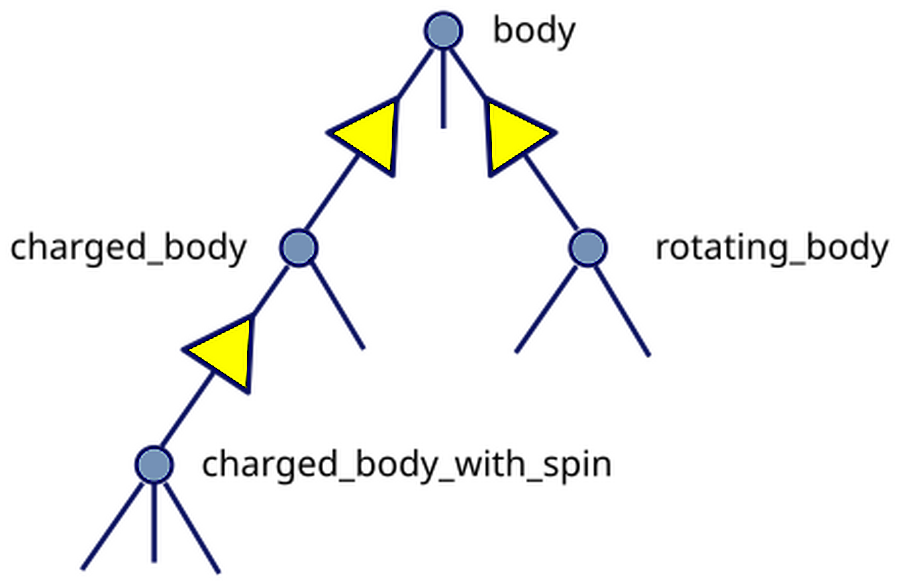
\includegraphics[width=8cm,height=\textheight,keepaspectratio]{Inheritance_diagram.svg.png}
\caption{~}
\end{figure}

An object of type \passthrough{\lstinline!body!} is \textbf{type
compatible} with both \passthrough{\lstinline!a\_proton!} and
\passthrough{\lstinline!a\_mutilated\_proton!}, so any of these two can,
for example, appear in a call to the procedure
\passthrough{\lstinline!kick!}.

\section{Polymorphism}\label{polymorphism}

\subsection{\texorpdfstring{Declaring entities with
\texttt{CLASS}}{Declaring entities with CLASS}}\label{declaring-entities-with-class}

By declaring an object with the \passthrough{\lstinline!CLASS!} instead
of the \passthrough{\lstinline!TYPE!} specifier, is is possible to defer
the actual type that an object has to be determined when the program
executes, or even have the actual type change during program execution.
Such an object is designated as being \textbf{polymorphic}. To be
polymorphic, an object must fulfill one of the following prerequisites:

\begin{itemize}
\tightlist
\item
  it has the \passthrough{\lstinline!POINTER!} attribute,
\item
  it has the \passthrough{\lstinline!ALLOCATABLE!} attribute, or
\item
  it is a dummy argument (with or without a
  \passthrough{\lstinline!POINTER!} or
  \passthrough{\lstinline!ALLOCATABLE!} attribute).
\end{itemize}

For example, the typed alllocation statement executed on a polymorphic
allocatable object

\begin{lstlisting}
CLASS(body), ALLOCATABLE :: a_polymorphic_body
:
ALLOCATE( charged_body :: a_polymorphic_body )
\end{lstlisting}

causes the object \passthrough{\lstinline!a\_polymorphic\_body!} that
has the \textbf{declared} type \passthrough{\lstinline!body!} to be
allocated with the \textbf{dynamic} type
\passthrough{\lstinline!charged\_body!}; in Fortran nomenclature, the
latter term denotes what was referred to above as ``actual'' type.

For an unallocated allocatable or a disassociated pointer the dynamic
type is considered to be the same as the declared type, although this is
only useful in very few contexts that do not require the object to be
allocated or associated.

\subsection{Run-time type and class
identification}\label{run-time-type-and-class-identification}

Within the scope of the object's declaration, only the components of its
declared type are accessible. Also, I/O operations on a polymorphic
object are not permitted, unless UDDTIO routines have been defined. One
way to obtain access to the complete object is to use a construct that
permits \textbf{run-time type identification} (not a Fortran term),
\passthrough{\lstinline!SELECT TYPE!}. For example, the I/O statements
in

\begin{lstlisting}
SELECT TYPE (a_polymorphic_body)
TYPE IS (body)
   WRITE(*,*) 'object of type body has value        ', a_polymorphic_body
TYPE IS (charged_body)
   WRITE(*,*) 'object of type charged_body has value', a_polymorphic_body
CLASS default
   ERROR STOP 'Type extension unsupported in this construct'
END SELECT
\end{lstlisting}

are permitted, since inside the block for each \textbf{type guard} the
object is non-polymorphic and of the specified type. At most one type
guard can match the object's type, and the corresponding statements are
executed; otherwise the \passthrough{\lstinline!CLASS default!} section
is executed (and the object remains polymorphic there). A disadvantage
of using \passthrough{\lstinline!SELECT TYPE!} is that it needs to be
appropriately updated whenever an additional type extension is defined;
apart from the maintenance effort this also requires access to all
source code that contain a relevant instance of the construct. For this
reason, type-bound procedures (to be discussed) should be preferably
used to gain access to additional type components.

For updates of the \passthrough{\lstinline!charge!} component of a
\passthrough{\lstinline!charged\_body!} object, one now could consider
the following:

\begin{lstlisting}
SUBROUTINE recharge(a_charged_body, dq)
   TYPE(charged_body), INTENT(inout) :: a_charged_body
   REAL, INTENT(in) :: dq

   a_charged_body%charge = a_charged_body%charge + dq
END SUBROUTINE
\end{lstlisting}

However, invoking this subroutine in the usual Fortran 95 style will not
work for the variable \passthrough{\lstinline!a\_polymorphic\_body!},
since it violates the rule that the dummy argument's declared type must
be type compatible with the actual argument's declared type. One can
work around this by using a \passthrough{\lstinline!SELECT TYPE!}
construct with \textbf{run-time class identification} (not a Fortran
term), based on writing \textbf{class guards} instead of type guards:

\begin{lstlisting}
SELECT TYPE (a_polymorphic_body)
CLASS IS (charged_body)  ! new declared type for a_polymorphic_body
   CALL recharge(a_polymorphic_body, dq=1.0e-5)
CLASS default
   WRITE(*,*) 'INFO: object a_polymorphic_body was not modified.'
END SELECT
\end{lstlisting}

The \passthrough{\lstinline!recharge!} procedure will then be invoked if
the dynamic type of \passthrough{\lstinline!a\_polymorphic\_body!} is
\passthrough{\lstinline!charged\_body!} or an extension of it. The
object remains polymorphic inside the class guard, only its declared
type changes to that specified in the guard. Unless the ``lifted''
declared type of interest is already otherwise known from the context,
or handling the \passthrough{\lstinline!CLASS default!} fall-through is
straightforward, this is not in general a desirable way of dealing with
class mismatches.

It is permitted to mix type and class guards in a
\passthrough{\lstinline!SELECT TYPE!} construct; in that case, a type
guard has precedence over a class guard specifying the same type with
respect to selection of the guarded statements to be executed.

\subsection{Unlimited polymorphic
objects}\label{unlimited-polymorphic-objects}

A special case of polymorphism is that an object can be
\textbf{unlimited polymorphic}. Such an object, declared with
\passthrough{\lstinline!CLASS(*)!}, can be of any dynamic type
(intrinsic type, extensible derived type,
\passthrough{\lstinline!SEQUENCE!} or \passthrough{\lstinline!BIND(C)!}
derived type), as illustrated by the following statements:

\begin{lstlisting}
CLASS(*), ALLOCATABLE :: a_unlimited  ! has no declared type, so any type is an extension

ALLOCATE( a_unlimited, source=2.5E4)  ! dynamic type becomes real

SELECT TYPE ( a_unlimited )
TYPE IS (REAL)
   WRITE(*,*) 'a_unlimited is of intrinsic real type with value ', a_unlimited
END SELECT

DEALLOCATE( a_unlimited )
ALLOCATE( a_unlimited, source=a_proton) )  ! dynamic type becomes charged_body

SELECT TYPE ( a_unlimited )
TYPE IS (charged_body)
   WRITE(*,*) 'a_unlimited is a charged_body with value ', a_unlimited
END SELECT
\end{lstlisting}

Accessing the object's data \emph{always} needs a
\passthrough{\lstinline!SELECT TYPE!} construct; type guards in the
construct can in this case might not only refer to extensible types, but
also to intrinsic types. However, for \passthrough{\lstinline!SEQUENCE!}
or \passthrough{\lstinline!BIND(C)!} derived types, no type resolution
is possible - these always fall through to a
\passthrough{\lstinline!CLASS default!} guard, if present; use of
unlimited polymorphic objects to store values of such types is therefore
considered unsafe.

In this context, allocation with \passthrough{\lstinline!source=!}
allocates the target object to the source object's dynamic type before
copying its value to the target object. If the source object's data is
not needed, \passthrough{\lstinline!mold=!} can be used instead. Sourced
allocation becomes a powerful tool, since the dynamic type of the source
object need not be known in the scoping unit within which the allocation
is executed.

Type components with the \passthrough{\lstinline!POINTER!} or
\passthrough{\lstinline!ALLOCATABLE!} attribute can be unlimited
polymorphic, enabling the construction of generic and potentially
inhomogeneous container-like types. As an illustration of this, a
supporting type for the purpose of holding data targeted for
manipulation of other objects is presented; its definition (placed in
the module \passthrough{\lstinline!mod\_utility\_types!}) reads

\begin{lstlisting}
TYPE :: any_object
   CHARACTER(len=:), ALLOCATABLE :: description
   CLASS(*), ALLOCATABLE :: value(:)
   INTEGER, ALLOCATABLE :: shape(:)
END TYPE
\end{lstlisting}

where \passthrough{\lstinline!description!} will refer to the property
that needs updating, and \passthrough{\lstinline!value!} will contain
the data to be used for the transaction. Because the
\passthrough{\lstinline!value!} component should be able to represent
any type, it is declared as being unlimited polymorphic. Because the
\passthrough{\lstinline!value!} component might hold data needed to
produce an array of arbitrary shape, the additional
\passthrough{\lstinline!shape!} component is supplied, but its use is
really only necessary if objects of rank at least 2 must be dealt with.
The structure constructor for that type has been overloaded to work
around compiler bugs and make handling of scalar data easier. The
following example illustrates how to establish a simple interface for
setting components of a structure:

\begin{lstlisting}
MODULE mod_wtype
   USE mod_utility_types, ONLY : initialize => any_object

   TYPE :: wtype
      PRIVATE
      INTEGER :: nonzeros = -1
      REAL, ALLOCATABLE :: w(:,:)
   END TYPE wtype
CONTAINS
   SUBROUTINE setup_wtype(a_wtype, a_component)
      ! in-place setting to avoid memory bursts for large objects
      TYPE(wtype), INTENT(inout) :: a_wtype
      TYPE(initialize), INTENT(in), TARGET :: a_component
      INTEGER :: wsize
      REAL, POINTER :: pw(:,:)

      SELECT CASE (a_component%description)
      CASE ("nonzeros")
         IF ( allocated(a_component%value) ) THEN
            SELECT TYPE ( nonzeros => a_component%value(1) )
            TYPE IS (INTEGER)
               a_wtype%nonzeros = nonzeros
            END SELECT
         END IF
      CASE ("w")
         IF ( allocated(a_component%value) .AND. allocated(a_component%shape) ) THEN
            wsize = size(a_component%value)
            IF ( wsize >= product(a_component%shape) ) THEN
               SELECT TYPE ( w => a_component%value )
               TYPE IS (REAL)
                  pw(1:a_component%shape(1), 1:a_component%shape(2)) => w
                  a_wtype%w = pw
               END SELECT
            END IF
         END IF
      END SELECT
   END SUBROUTINE setup_wtype
   :
END MODULE
\end{lstlisting}

\textbf{Notes:}

\begin{itemize}
\tightlist
\item
  Having this simple interface at the cost of significant additional
  setup code might at first sight appear frivolous; however, once type
  extension is used on a larger scale, setting or modifying further
  components in the conventional way becomes rather irksome without a
  concept like that above, especially if \hyperref[sec:tbp]{type-bound
  procedures} with a simple \emph{and} uniform interface must be
  implemented;
\item
  The object \passthrough{\lstinline!a\_wtype!} remains unchanged in
  case an unsuitable value is provided for
  \passthrough{\lstinline!a\_component!}. One could add explicit error
  handling, but for these examples this is considered an unnecessary
  complication;
\item
  The permitted values for the \passthrough{\lstinline!initialize!}
  object should be documented for each procedure that takes such an
  object;
\item
  Because access to \passthrough{\lstinline!a\_component!} within
  \passthrough{\lstinline!SELECT TYPE!} is via a type component, one is
  obliged to introduce an associate name for the latter. The language
  rules only permit omitting the associate name for named variables, and
  subobjects are not named variables;
\item
  A \textbf{rank-changing pointer assignment} is used to transform the
  rank-1 \passthrough{\lstinline!a\_component\%value!} array to an
  object that can be assigned to a rank-2
  \passthrough{\lstinline!a\_wtype\%w!} array; this works because the
  right-hand side is a rank-1 object; for rank-2 and higher the
  rank-changing pointer assignment will only work if the target assigned
  to is a \textbf{simply contiguous array designator} (a topic not
  covered here). Note that in this context, the
  \passthrough{\lstinline!reshape!} intrinsic cannot be used because it
  requires the size of its \passthrough{\lstinline!shape!} argument to
  be a constant.
\end{itemize}

The program invoking the \passthrough{\lstinline!setup\_wtype!}
procedure might do so as follows, to set up a
\passthrough{\lstinline!wtype!} object:

\begin{lstlisting}
USE mod_wtype
TYPE(initialize) :: c_nz, c_w
TYPE(wtype) :: my_wtype
INTEGER :: i, j
INTEGER :: ndim

ndim = ...

ASSOCIATE ( my_data => [ ((real (max(0, min(i-j+2, j-i+2))), j=1, ndim), i=1, ndim) ] )
   c_nz = initialize("nonzeros", count(my_data /= 0))
   c_w = initialize("w", my_data, [ ndim, ndim ] )
END ASSOCIATE

CALL setup_wtype(my_wtype, c_nz)
CALL setup_wtype(my_wtype, c_w)
\end{lstlisting}

\section{Type-bound procedures (TBP)}\label{sec:tbp}

To resolve the class mismatch issues arising from the use of polymorphic
objects, one needs a language mechanism for making a run-time decision
on a procedure invocation that depends on the dynamic type of a
polymorphic object. This can be achieved by binding a procedure to a
type in the type definition via a \passthrough{\lstinline!PROCEDURE!}
statement in the type's \passthrough{\lstinline!CONTAINS!} part.

For the type \passthrough{\lstinline!body!}, the augmented type
definition reads

\begin{lstlisting}
TYPE :: body
   REAL :: mass
   REAL :: pos(3), vel(3)
CONTAINS
   PROCEDURE :: update => update_body
END TYPE
\end{lstlisting}

This does not impact how the structure constructor is used; for this,
only the specifications before the \passthrough{\lstinline!CONTAINS!}
statement are relevant. To establish a simple and uniform interface for
object updates, the procedure \passthrough{\lstinline!update\_body!}
makes use of the \passthrough{\lstinline!any\_object!} type discussed
earlier, which in view of the context is locally renamed to
\passthrough{\lstinline!change!}:

\begin{lstlisting}
SUBROUTINE update_body(a_body, a_change)
   CLASS(body), INTENT(inout) :: a_body
   TYPE(change), INTENT(in) :: a_change
   IF ( allocated(a_change%description) .AND. allocated(a_change%value) ) THEN
     SELECT CASE ( trim(a_change%description) )
     CASE ('mass')
        SELECT TYPE ( delta => a_change%value(1) )
        TYPE IS (real)
           CALL accrete(a_body, delta)
        END SELECT
     CASE ('momentum')
        SELECT TYPE ( delta => a_change%value )
        TYPE IS (real)
           IF ( size(delta) >= 3 ) CALL kick(a_body, delta(1:3))
        END SELECT
     CASE ('position')
        SELECT TYPE ( delta => a_change%value )
        TYPE IS (real)
           IF ( size(delta) >= 3) a_body%pos = a_body%pos + delta(1:3)
        END SELECT
     END SELECT
   END IF
END SUBROUTINE
\end{lstlisting}

In its interface, the \textbf{passed object}
\passthrough{\lstinline!a\_body!} must be declared to be a polymorphic
scalar, with its declared type being the one the procedure has been
bound to. The implementation reuses existing code where possible (very
simple in this example, but this is of course not generally the case),
to avoid the need for extensive revalidation.

Invocation of the procedure could be done in the usual manner, but the
preferred style, especially in the case that the actual argument is
polymorphic, is to do it through the object itself:

\begin{lstlisting}
TYPE(change) ::  dx
:
dx = change(description='mass', value=[0.0, 2.0, 0.0])

CALL my_basketball%update(dx) ! invokes update_body(my_basketball, dx)
\end{lstlisting}

For polymorphic objects, the procedure
\passthrough{\lstinline!update\_body!} will be invoked if the dynamic
type of the object is \passthrough{\lstinline!body!} (this might not be
true if the dynamic type is an extension, as we shall see).

The invocation can also be done with non-polymorphic objects; in this
case, the binding could (in principle) be determined at compilation
time, potentially saving some call overhead. Note that the passed object
dummy is not permitted to be allocatable or a pointer, which facilitates
this usage.

So far this is not particularly interesting; the key thing is what
happens once we turn to type extensions. For example, to enable
modification of the \passthrough{\lstinline!charge!} component (in
addition to that of other components) of an object of dynamic type
\passthrough{\lstinline!charged\_body!}, it is possible to
\textbf{override} the parent type's bound procedure:

\begin{lstlisting}
TYPE, EXTENDS(body) :: charged_body
   REAL :: charge
CONTAINS
   PROCEDURE :: update => update_charged_body
END TYPE
\end{lstlisting}

with the procedure defined as follows:

\begin{lstlisting}
SUBROUTINE update_charged_body(a_body, a_change)
   CLASS(charged_body) :: a_body
   TYPE(change) :: a_change

   IF ( allocated(a_change%description) .AND. allocated(a_change%value) ) THEN
      SELECT CASE ( trim(a_change%description) )
      CASE ('charge')
         SELECT TYPE ( delta => a_change%value(1) )
         TYPE IS (real)
            a_body%charge = a_body%charge + delta
         END SELECT
      CASE default
         CALL a_body%body%update(a_change)
         ! assure that a change to a parent component is dealt with
      END SELECT
   END IF
END SUBROUTINE
\end{lstlisting}

The overriding procedure must use the same interface as the overridden
procedure, except that the passed object is declared to be of the
extended type; even the argument keywords must be the same. Once the
override has been defined, the call through an object of dynamic type
\passthrough{\lstinline!charged\_body!} will be dispatched to
\passthrough{\lstinline!update\_charged\_body!}:

\begin{lstlisting}
TYPE(change) ::  dc, dp
CLASS(body), ALLOCATABLE :: my_polymorphic_body

my_polymorphic_body = charged_body(mass=1.5, pos=[0.,0.,0.], &
                                   vel=[2.,0.,0.], charge=2.41E-5)
!  the above statement auto-allocates the left hand side
dc = change(description='charge', value=5.0E-6)
dp = change(description='momentum', value=[-1.0,1.0,0.0])

! both the following dispatch to update_charged_body
CALL my_polymorphic_body%update(dc)
CALL my_polymorphic_body%update(dp)
\end{lstlisting}

\textbf{Notes:}

\begin{itemize}
\tightlist
\item
  for the above example, direct invocation of the procedure
  \passthrough{\lstinline!update\_charged\_body!} is not possible (as
  already noted earlier);
\item
  the second TBP call illustrates the invocation of the parent object
  update from \passthrough{\lstinline!update\_charged\_body!}. Without
  this, changes that impact the parent object would not be done. By
  implementing this consistency of behaviour, the programmer assures
  that the inheritance hierarchy adheres to the
  \href{https://en.wikipedia.org/wiki/Liskov_substitution_principle}{Liskov
  substitution principle};
\item
  to enforce using the TBP calls in a use association context, the
  module procedures that implement them can be made
  \passthrough{\lstinline!PRIVATE!}. The accessibility of the TBP itself
  is determined by the attribute for it (default is
  \passthrough{\lstinline!PUBLIC!}) in the type definition;
\item
  the programmer can prevent overriding of a binding by declaring it to
  be \passthrough{\lstinline!NON\_OVERRIDABLE!}; its implementation then
  is regarded as valid for all conceivable extension types.
\end{itemize}

\section{Abstract types and
interfaces}\label{abstract-types-and-interfaces}

The \passthrough{\lstinline!sortable!} type used for demonstrating the
\passthrough{\lstinline!sortable\_list!} functionality in the
\hyperref[sec:oop_techniques]{object-based chapter's} example was set up
as a fixed container-like type. It is desirable to be able to use the
list machinery more flexibly i.e., for any type that supports the
``less-than'' comparison. This can be achieved by introducing an
\textbf{abstract type}

\begin{lstlisting}
TYPE, ABSTRACT :: sortable
CONTAINS
   PROCEDURE(compare), DEFERRED :: less_than
   ! ... more to follow
END TYPE
\end{lstlisting}

with a \textbf{deferred binding}. It is not possible to create an object
whose dynamic type is abstract, or a non-polymorphic object of abstract
type. For this reason, the deferred binding cannot represent an existing
procedure, but is characterized by an \textbf{abstract interface}:

\begin{lstlisting}
ABSTRACT INTERFACE
   PURE LOGICAL FUNCTION compare(s1, s2)
      IMPORT :: sortable
      CLASS(sortable), INTENT(in) :: s1, s2
      ! dispatch is via the first argument
   END FUNCTION
END INTERFACE
\end{lstlisting}

The \passthrough{\lstinline!IMPORT!} statement is required to give the
interface access to the type defined in its host. Furthermore, an
override of the structure constructor will be needed

\begin{lstlisting}
INTERFACE sortable
   PROCEDURE :: create_sortable
END INTERFACE
\end{lstlisting}

that permits creation of polymorphic \passthrough{\lstinline!sortable!}
objects. The details of this will be described later (since, indeed, a
devil lurks in these details). Note that the above combined use of
abstract types and interfaces is also known under the (non-Fortran) term
\textbf{interface class}.

This framework permits the programmer to implement the following
programming technique, which is also known as \textbf{dependency
inversion} (not a Fortran term):

\begin{enumerate}
\def\labelenumi{\arabic{enumi}.}
\item
  Any machinery that makes use of polymorphic
  \passthrough{\lstinline!sortable!} objects is made to only refer to
  the above abstractions. For example, the definition of the
  \passthrough{\lstinline!sorted\_list!} type could be adapted to read

\begin{lstlisting}
TYPE, PUBLIC :: sorted_list
   PRIVATE
   CLASS(sortable), ALLOCATABLE :: data
   ! changed to refer to abstract type
   TYPE(sorted_list), POINTER :: next => null()
CONTAINS
   FINAL :: delete_sorted_list
END TYPE
\end{lstlisting}
\end{enumerate}

The advantage of this is that no change to the preexisting machinery
will be needed whenever a programmer decides to add an extension type as
outlined in 2. below.

\begin{enumerate}
\def\labelenumi{\arabic{enumi}.}
\setcounter{enumi}{1}
\item
  For a concrete realization of a \passthrough{\lstinline!sortable!}
  object, the programmer needs to create a type extension, for example

\begin{lstlisting}
TYPE, PUBLIC, EXTENDS(sortable) :: sortable_string
   CHARACTER(len=:), ALLOCATABLE :: string
CONTAINS
   PROCEDURE :: less_than => less_than_string
END TYPE
\end{lstlisting}
\end{enumerate}

including an \emph{obligatory} implementation
\passthrough{\lstinline!less\_than\_string!} of an overriding TBP for
the deferred binding. The constructor function (promised earlier, but
not yet delivered) also needs to be updated to enable creation of
objects of the extended type.

\section{Generic type-bound procedures and operator
overloading}\label{generic-type-bound-procedures-and-operator-overloading}

As a convenience, use of an overloading for the comparison operator
``\textless{}'' can be provided by creating a \textbf{generic}
type-bound procedure:

\begin{lstlisting}
TYPE, ABSTRACT :: sortable
CONTAINS
   PROCEDURE(compare), DEFERRED :: less_than
   GENERIC :: OPERATOR(<) => less_than
END TYPE
\end{lstlisting}

which means that when a statement involving a comparison expression

\begin{lstlisting}
CLASS(sortable), ALLOCATABLE :: s1, s2

s1 = sortable( ... )
s2 = sortable( ... )

IF ( s1 < s2 ) THEN
   ...
END IF
\end{lstlisting}

is executed, the overridden type-bound procedure bound to the first
operand will be invoked to evaluate the expression. It is not necessary
to re-specify the \passthrough{\lstinline!GENERIC!} clause in any type
extensions; the dispatch will automatically select the overridden
procedure.

Named generic type-bound procedures that do not overload existing
operations can also be defined; an example for this is given in the
section ``\hyperref[sec:functions_with_parameters]{Functions with
parameters}''. The rules for generic resolution work similar as for
nonpolymorphic generic procedure interfaces, with the additional
restriction that polymorphic dummy arguments that are related by
inheritance cannot be distinguished for the purpose of compile-time
resolution to a specific procedure.

\section{Completing the dependency
inversion}\label{completing-the-dependency-inversion}

\subsection{Discussion of structural
dependencies}\label{discussion-of-structural-dependencies}

When implementing the above concept, typically a separate module, say
\passthrough{\lstinline!mod\_sortable\_extensions!}, is created for some
or all of the extension types of \passthrough{\lstinline!sortable!}. The
motivations for this can be:

\begin{itemize}
\tightlist
\item
  avoid recompilation of any machinery that makes use of the
  \passthrough{\lstinline!mod\_sortable!} module;
\item
  the source code of \passthrough{\lstinline!mod\_sortable!} might not
  be readily modifiable;
\item
  prevent \passthrough{\lstinline!mod\_sortable!} from turning into a
  monster module in case large concepts are implemented through
  extension types, or many extension types are created.
\end{itemize}

The implementation of the constructor will need to use associate
\passthrough{\lstinline!mod\_sortable\_extensions!} since it needs to be
able to create objects of the types defined there. On the other hand,
the interface to the constructor needs to be visible in
\passthrough{\lstinline!mod\_sortable!}, since the machinery that
depends on it must be able to call it. As a consequence, one would end
up with a circular \passthrough{\lstinline!USE!} dependency between the
two modules, which is prohibited.

\subsection{Using submodules to break dependency
cycles}\label{using-submodules-to-break-dependency-cycles}

To deal with such a situation (among others), the concept of
\textbf{submodule} is available. This is a type of program unit that
serves as an extension to an existing module (or submodule), to which it
has access by host association. Furthermore, submodules allow the
programmer to separate interfaces from implementations; the former are
defined in the parent program unit (i.e., the program unit of which the
submodule is an extension), the latter in the submodule itself.

For the constructor function, the following interface block can be
declared in \passthrough{\lstinline!mod\_sortable!}:

\begin{lstlisting}
INTERFACE
   MODULE FUNCTION create_sortable(init) RESULT(r)
      CLASS(sortable), ALLOCATABLE :: r
      TYPE(initialize), INTENT(in) :: init
   END FUNCTION
END INTERFACE
\end{lstlisting}

The special notation \passthrough{\lstinline!MODULE FUNCTION!} (or
\passthrough{\lstinline!MODULE SUBROUTINE!} for a subroutine) tells the
compiler that the implementation is deferred to a submodule.

\textbf{Notes:}

\begin{itemize}
\tightlist
\item
  the above interface requires no reference to any entities contained in
  \passthrough{\lstinline!mod\_sortable\_extensions!};
\item
  consistent with this, the variable representing the function result is
  an allocatable polymorphic object of the abstract type;
\item
  an \passthrough{\lstinline!IMPORT!} statement is not obligatory in
  separate module procedure interfaces, although it is permitted
  (compiler support assumed!), primarily for the purpose of fine-grain
  control of host access;
\item
  the type \passthrough{\lstinline!initialize!} is, again, a renamed
  version of the \passthrough{\lstinline!any\_object!} type referred to
  earlier.
\end{itemize}

\subsection{Implementation of the
constructor}\label{implementation-of-the-constructor}

The submodule containing the implementation then reads as follows:

\begin{lstlisting}
SUBMODULE (mod_sortable) smod_constructor
CONTAINS
   MODULE PROCEDURE create_sortable
      USE mod_sortable_extensions, ONLY : sortable_string

      IF ( allocated(init%description) .AND. allocated(init%value) ) THEN
         SELECT CASE (init%description)
         CASE ('sortable_string')
            SELECT TYPE ( value => init%value(1) )
            TYPE IS (CHARACTER(len=*))
               ALLOCATE( r, source=sortable_string(value) )
            END SELECT
         END SELECT
      END IF
   END PROCEDURE
END SUBMODULE
\end{lstlisting}

\textbf{Notes:}

\begin{itemize}
\tightlist
\item
  The interface for the separate module procedures is omitted, since it
  can be deduced from its specification in the parent module. However,
  alternative syntax exists that replicates the interface (but this is
  not shown here);
\item
  the effect of the \passthrough{\lstinline!ONLY!} clause is to suppress
  use access to any entity of the parent program unit (which would be
  indirectly established). This is because use association overrides
  host association, which may cause undesirable side effects;
\item
  submodules additionally can contain specifications (before the
  \passthrough{\lstinline!CONTAINS!} statement), as well as local
  submodule procedures. All these are only accessible from the submodule
  (and its descendant submodules, if any);
\item
  the naming scheme for a submodule always references the direct parent.
  For submodules of submodules, the scheme is
  \passthrough{\lstinline!SUBMODULE (<parent module>:<parent submodule>) <submodule\_name>!}
  and the names of submodules of a given module must be unique.
\end{itemize}

\subsection{Diagramming the dependencies between program
units}\label{diagramming-the-dependencies-between-program-units}

The following diagram shows the use and host association relationships
between the modules (blue boxes), the submodule (green box), and a main
program unit (orange box) for this example:

\begin{figure}
\centering
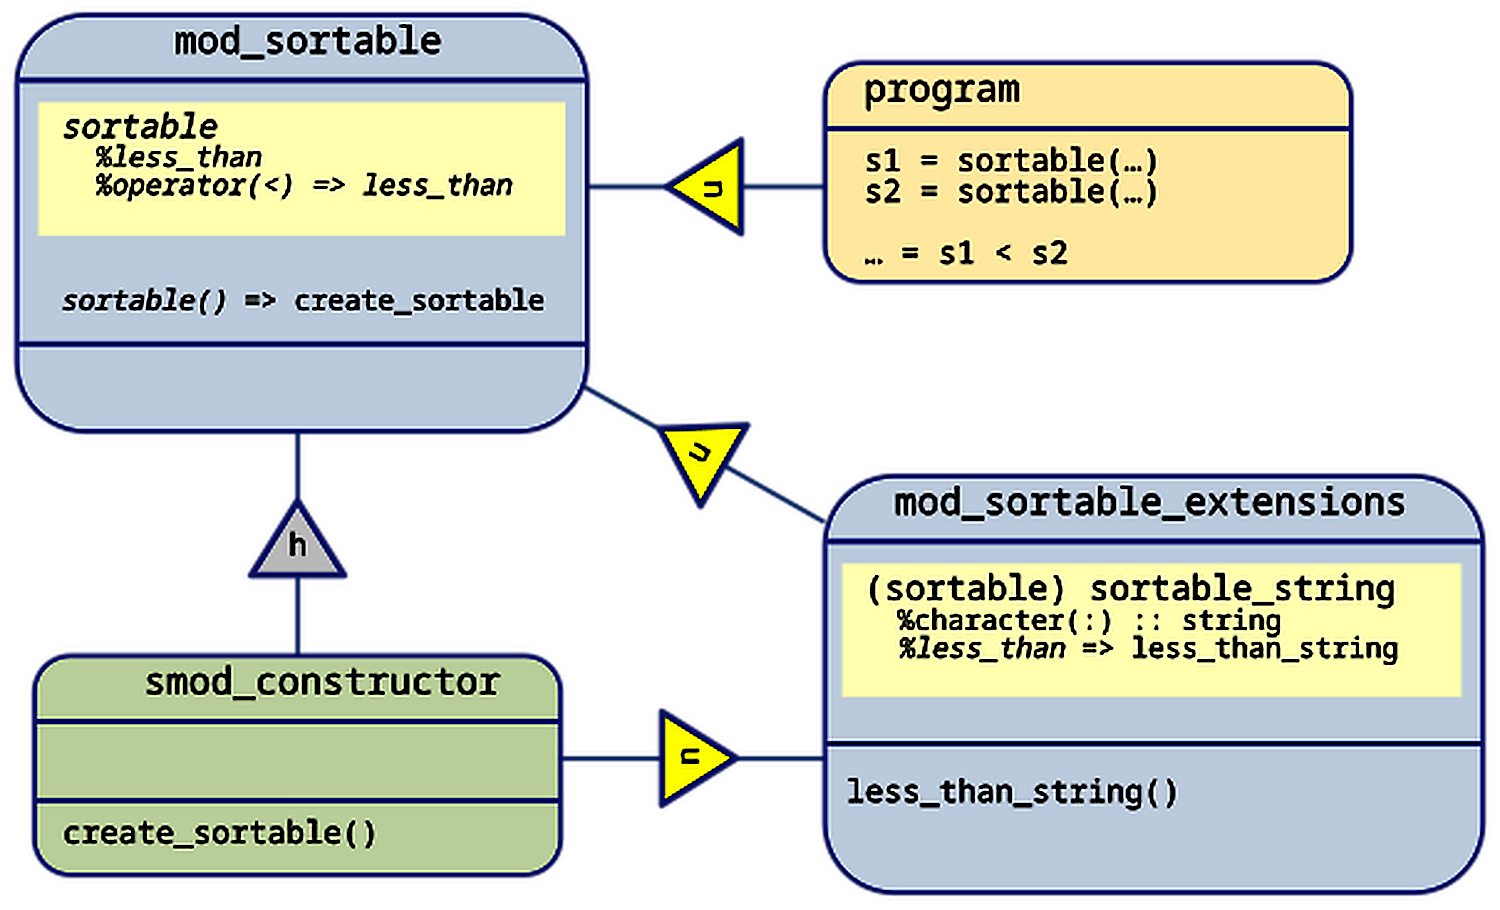
\includegraphics[width=8cm,height=\textheight,keepaspectratio]{Dependency_inversion.svg.png}
\caption{Dependencies between program units implementing and using an
interface class}
\end{figure}

The small triangles in the diagram refer to use (``u'') association and
host (``h'') association, respectively. The separation of the
constructor's interface from its implementation leads to avoidance of
circular \passthrough{\lstinline!USE!} references (the lower two ``u''
triangles in the diagram).

The compilation order for separate files would be:

\begin{enumerate}
\def\labelenumi{\arabic{enumi}.}
\tightlist
\item
  \passthrough{\lstinline!mod\_sortable!}
\item
  \passthrough{\lstinline!program!} and
  \passthrough{\lstinline!mod\_sortable\_extensions!}, independently
\item
  \passthrough{\lstinline!smod\_constructor!}
\end{enumerate}

\section{Performance and ease of use}\label{performance-and-ease-of-use}

\section{Functions with parameters}\label{sec:functions_with_parameters}

\subsection{A type definition for invocation of a general
function}\label{a-type-definition-for-invocation-of-a-general-function}

In scientific applications, a commonly occurring requirement is the need
to evaluate functions that depend on additional parameters, apart from
their real-valued argument. For example, an application might need the
value of spherical Bessel function \(x \mapsto j_l(q \, x)\) for
independently specified integer values of \(l\) and real values of
\(q\). More generally, one can consider a real-valued mapping

\(\Re \ni x \mapsto f_\lambda(x) \quad (\lambda \in \Omega)\),

where the parameter value \(\lambda\) can be from some arbitrary set.
This section presents a way for handling this programmatically, using
the object-oriented features of Fortran. We start with the outline for a
type definition of sufficient generality:

\begin{lstlisting}
TYPE, PUBLIC :: pfunc_type
   PRIVATE
   PROCEDURE(pfunc), POINTER, NOPASS :: fp => null()
   : ! shown later
   CLASS(*), ALLOCATABLE :: param
CONTAINS
   : ! shown later
END type pfunc_type

ABSTRACT INTERFACE
   PURE REAL FUNCTION pfunc(x, param)
      REAL, INTENT(in) :: x
      CLASS(*), INTENT(in), OPTIONAL :: param
   END FUNCTION pfunc
END INTERFACE
\end{lstlisting}

It supplies

\begin{itemize}
\tightlist
\item
  a \textbf{procedure pointer} component with an abstract interface that
  reflects the above mapping;
\item
  an unlimited polymorphic parameter component, to keep all things in
  one place.
\end{itemize}

Notionally, one could invoke a properly set up
\passthrough{\lstinline!pfunc\_type!} object through

\begin{lstlisting}
TYPE(pfunc_type) :: pfunc_obj
REAL :: x

pfunc_obj = pfunc_type(psin, 2)
! definitions of procedure and data object discussed further below
x = ...

WRITE(*,*) 'Function value is ', pfunc_obj%fp(x, pfunc_obj%param)
\end{lstlisting}

Use of a procedure pointer reflects the fact that each
\passthrough{\lstinline!pfunc\_type!} object will want to associate its
individual target function; this is sometimes also referred to as an
\textbf{object-bound procedure}. The \passthrough{\lstinline!NOPASS!}
attribute in the type definition is needed because otherwise (analogous
to what we saw for the earlier type-bound procedure examples), the
object through which the invocation is done would be obliged to appear
as a first argument in the abstract interface
\passthrough{\lstinline!pfunc!}; this would constitute an additional
imposition on the implementation of the supplied functions. On the other
hand, the invocation needs to explicitly specify the
\passthrough{\lstinline!param!} component, making it a bit unwieldy; the
use of \passthrough{\lstinline!pfunc\_type!} objects will be simplified
as we go on.

\subsection{Performance issues arising from object-oriented
programming}\label{performance-issues-arising-from-object-oriented-programming}

Let us look at a target function implementation, in form of a trivial
example \(\sin(\lambda x)\):

\begin{lstlisting}
PURE REAL FUNCTION psin(x, param)
   REAL, INTENT(in) :: x
   CLASS(*), INTENT(in), OPTIONAL :: param
   REAL :: factor
   factor = 1.
   IF ( present(param) ) THEN
      SELECT TYPE ( param )
      TYPE IS (REAL)
         factor = param
      TYPE IS (INTEGER)
         factor = real(param)
      END SELECT
   END IF
   psin = sin(factor*x)
END FUNCTION psin
\end{lstlisting}

Given that an application is likely to request a large number of
function values, the following effects would ensue once for each
invocation:

\begin{itemize}
\tightlist
\item
  function call overhead, and
\item
  overhead of run-time type resolution.
\end{itemize}

The resulting performance impact is typical for object-oriented designs
that operate in multitudes on small objects. Making use of an
array-based version of the function

\begin{lstlisting}
PURE FUNCTION psin_array(x, param) RESULT(r)
   REAL, INTENT(in) :: x(:)
   REAL :: r(size(x))
   CLASS(*), INTENT(in), OPTIONAL :: param
   REAL :: factor
   factor = 1.
   IF ( present(param) ) THEN
      SELECT TYPE ( param )
      TYPE IS (REAL)
         factor = param
      TYPE IS (INTEGER)
         factor = real(param)
      END SELECT
   END IF
   r = sin(factor*x)  ! kernel
END FUNCTION psin_array
\end{lstlisting}

is desirable, since the overheads specified above only arise
\emph{once}, and the actual calculational code (marked ``kernel'' in the
above box) is amenable to array-related compiler optimizations (the
specifics of which depend on both hardware architecture and working set
size).

\subsection{Completing the function type
definition}\label{completing-the-function-type-definition}

The aim now is to proceed to a framework that permits to use both the
scalar and the array versions in a uniform way, thereby making life for
the clients that use the framework easy, while enabling performance
where it is needed.

The full definition of \passthrough{\lstinline!pfunc\_type!}, including
its referenced abstract interfaces, reads

\begin{lstlisting}
TYPE, PUBLIC :: pfunc_type
   PRIVATE
   PROCEDURE(pfunc), POINTER, NOPASS :: fp => null()
   PROCEDURE(pfunc_array), POINTER, NOPASS :: fp_array => null()
   CLASS(*), ALLOCATABLE :: param
CONTAINS
   PROCEDURE, PASS, PRIVATE, NON_OVERRIDABLE :: f_scalar, f_array
   GENERIC :: f => f_scalar, f_array
END type pfunc_type

ABSTRACT INTERFACE
   PURE REAL FUNCTION pfunc(x, param)
      REAL, INTENT(in) :: x
      CLASS(*), INTENT(in), OPTIONAL :: param
   END FUNCTION pfunc
   PURE FUNCTION pfunc_array(x, param) RESULT(r)
      REAL, INTENT(in) :: x(:)
      REAL :: r(size(x))
      CLASS(*), INTENT(in), OPTIONAL :: param
   END FUNCTION pfunc_array
END INTERFACE
\end{lstlisting}

Because we now have two procedure pointers in the type (only one of
which is used in each given object), it is advantageous to provide a
generic type-bound procedure \passthrough{\lstinline!f!} as a front end
for ease of use. The specifics \passthrough{\lstinline!f\_scalar!} and
\passthrough{\lstinline!f\_array!} for this read

\begin{lstlisting}
REAL FUNCTION f_scalar(this, x)
   CLASS(pfunc_type), INTENT(in) :: this
   REAL, INTENT(in) :: x

   IF ( associated(this%fp) ) THEN
      f_scalar = this%fp(x, this%param)
   ELSE IF ( associated(this%fp_array) ) THEN
      ASSOCIATE ( f_array => this%fp_array([x], this%param) )
         f_scalar = f_array(1)
      END ASSOCIATE
   ELSE
      ERROR STOP 'pfunc_type callback: uninitialized object'
   END IF
END FUNCTION f_scalar
FUNCTION f_array(this, x) RESULT(r)
   CLASS(pfunc_type), INTENT(in) :: this
   REAL, INTENT(in) :: x(:)
   REAL :: r(size(x))

   ! Note that support for the scalar version is omitted here, since
   ! the procedure call overhead, including type resolution, would
   ! significantly impact performance.
   IF ( associated(this%fp_array) ) THEN
      r = this%fp_array(x, this%param)
   ELSE
      ERROR STOP 'pfunc_type callback: uninitialized object'
   END IF
END FUNCTION f_array
\end{lstlisting}

The only way to invoke one of these (in a use association context) is
via the generic name, since the specific type-bound procedures have the
\passthrough{\lstinline!PRIVATE!} attribute; note that
\passthrough{\lstinline!pfunc\_type!} is not designed for being
extended. Disambiguation is by rank of \passthrough{\lstinline!x!}.

The structure constructor for the type is overloaded

\begin{lstlisting}
INTERFACE pfunc_type
   MODULE PROCEDURE create_pfunc_type
   MODULE PROCEDURE create_pfunc_type_array
END INTERFACE pfunc_type
\end{lstlisting}

with the following specific functions:

\begin{lstlisting}
TYPE(pfunc_type) FUNCTION create_pfunc_type(fp, param)
   PROCEDURE(pfunc) :: fp
   CLASS(*), INTENT(in), OPTIONAL :: param
   create_pfunc_type%fp => fp
   IF ( present(param) ) THEN
      ALLOCATE(create_pfunc_type%param, source=param)
   END IF
END FUNCTION create_pfunc_type
TYPE(pfunc_type) FUNCTION create_pfunc_type_array(fp_array, param)
   PROCEDURE(pfunc_array) :: fp_array
   CLASS(*), INTENT(in), OPTIONAL :: param
   create_pfunc_type_array%fp_array => fp_array
   IF ( present(param) ) THEN
      ALLOCATE(create_pfunc_type_array%param, source=param)
   END IF
END FUNCTION create_pfunc_type_array
\end{lstlisting}

Disambiguation is possible due to the sufficiently different interfaces
of the procedure arguments.

\subsection{Using the function type}\label{using-the-function-type}

With the already-shown implementations for the target functions
\passthrough{\lstinline!psin!} and
\passthrough{\lstinline!psin\_array!}, using this framework is
illustrated by the following:

\begin{lstlisting}
TYPE(pfunc_type) :: pfunc_obj
REAL, PARAMETER :: piby4 = atan(1.0), &
   piby4_arr(4) = [ piby4, 2.*piby4, 3.*piby4, 4.*piby4 ]

pfunc_obj = pfunc_type(psin, 2.)
WRITE(*,*) pfunc_obj%f(piby4)

pfunc_obj = pfunc_type(psin)
WRITE(*,*) pfunc_obj%f(piby4)

pfunc_obj = pfunc_type(psin_array, 2.)
WRITE(*,*) pfunc_obj%f(piby4_arr)
\end{lstlisting}

Omitting a \passthrough{\lstinline!param!} in a constructor is fine, as
long as the target functions cater for the dummy argument's
non-presence.

The framework's implementation makes use of the fact that an unallocated
actual argument associated with an \passthrough{\lstinline!OPTIONAL!}
dummy argument is considered not present. Once conditional expressions
are implemented in compilers, the code will be appropriately reworked,
since use of this feature is recommended against.

\section{Arrays of structures versus structures of
arrays}\label{arrays-of-structures-versus-structures-of-arrays}

Returning to our earlier example type body, the next idea would be to
simulate the dynamics of a large ensemble of bodies. A procedure

\begin{lstlisting}
SUBROUTINE propagate(bodies, delta_t, force_field)
   TYPE(body), INTENT(inout) :: bodies(:)
   REAL, INTENT(in) :: delta_t
   TYPE(field_type), INTENT(in) :: force_field
   :
END SUBROUTINE
\end{lstlisting}

might be supplied that modifies the components of all ensemble members,
for example as follows:

\begin{itemize}
\tightlist
\item
  \passthrough{\lstinline!\%pos!} \(\longrightarrow\)
  \passthrough{\lstinline!\%pos + delta\_t * \%vel!}
\item
  \passthrough{\lstinline!\%vel!} \(\longrightarrow\)
  \passthrough{\lstinline!\%vel + delta\_t * force / \%mass!}
\end{itemize}

where \passthrough{\lstinline!force!} results from evaluating
\passthrough{\lstinline!force\_field!} at the position of the ensemble
member.

\section{Comments on further language
features}\label{comments-on-further-language-features}

\subsection{Variations on the passed
object}\label{variations-on-the-passed-object}

All examples for type-bound procedures given up to now have the property
that the invoking object itself is passed as the first argument to the
bound procedure. However, this default behaviour can be modified by the
programmer

\begin{itemize}
\tightlist
\item
  either declaring the binding with a \passthrough{\lstinline!PASS!}
  attribute that references the specific (and of course appropriately
  declared) procedure argument the object of the bound type should be
  passed to,
\item
  or declaring the binding with a \passthrough{\lstinline!NOPASS!}
  attribute, in which case the object is not (implicitly) passed to the
  procedure at all in a TBP invocation.
\end{itemize}

\section{References}\label{references}

\end{document}
